\subsection{The application}

The deployed model is the Ridge pipeline refit on all 188 sales. The split existed to
obtain an unbiased error estimate, and once that is recorded there is no reason to
discard 30\% of the evidence. It is serialised to \texttt{src/model.joblib} with its column lists, so
the app builds feature rows from the definitions used in training.

\texttt{src/app.py} is a Streamlit prototype loading that bundle, offering a
single-property form and a CSV upload. Inputs are only fields readable off a listing,
including floor or land area, which can be left blank. Derived terms are
computed internally. The app exponentiates before display and reports
a $\pm 20\%$ band rather than a point estimate.

\begin{verbatim}
pip install -r requirements.txt
jupyter nbconvert --to notebook --execute --inplace notebooks/lab.ipynb
streamlit run src/app.py        # from the project root; serves localhost:8501
\end{verbatim}

The notebook must run first, since it writes \texttt{src/model.joblib}. Full instructions,
including rebuilding the dataset from the cached raw pages, are in \texttt{README.md}.

\begin{figure}[H]
\centering
\begin{subfigure}{0.49\textwidth}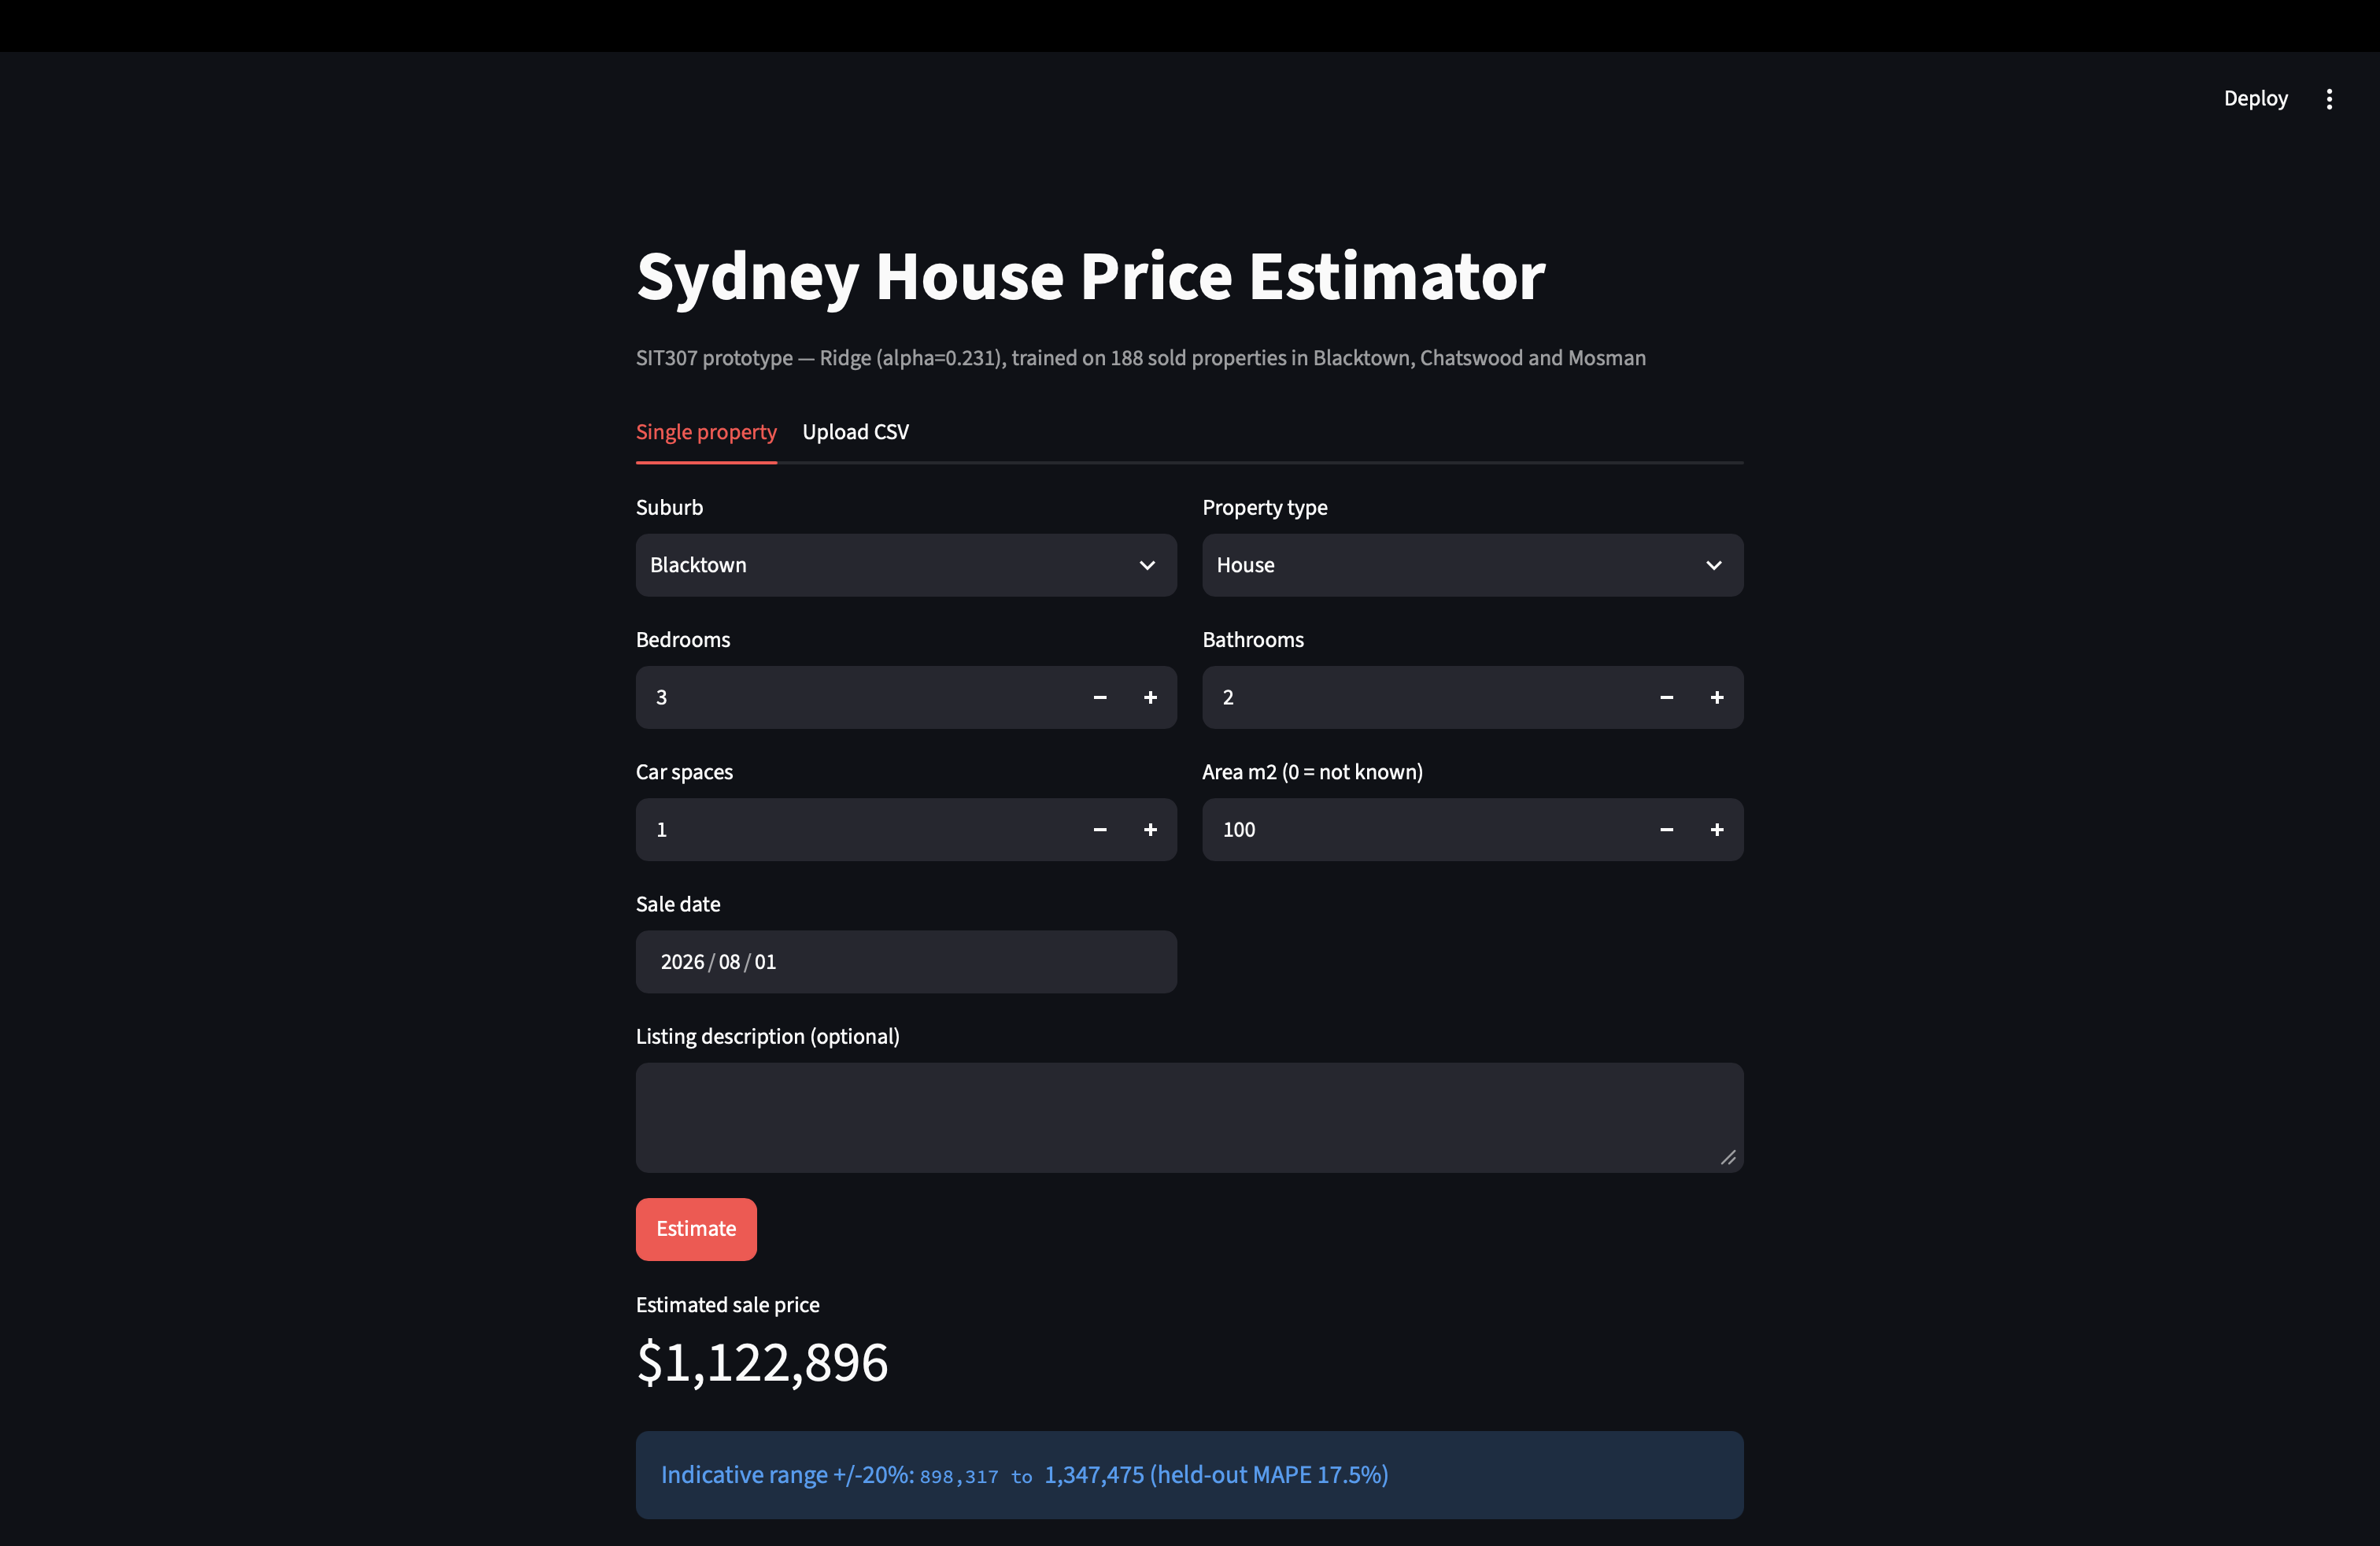
\includegraphics[width=\linewidth]{figures/p5_app_single.png}
\caption{Single-property estimate.}\end{subfigure}\hfill
\begin{subfigure}{0.49\textwidth}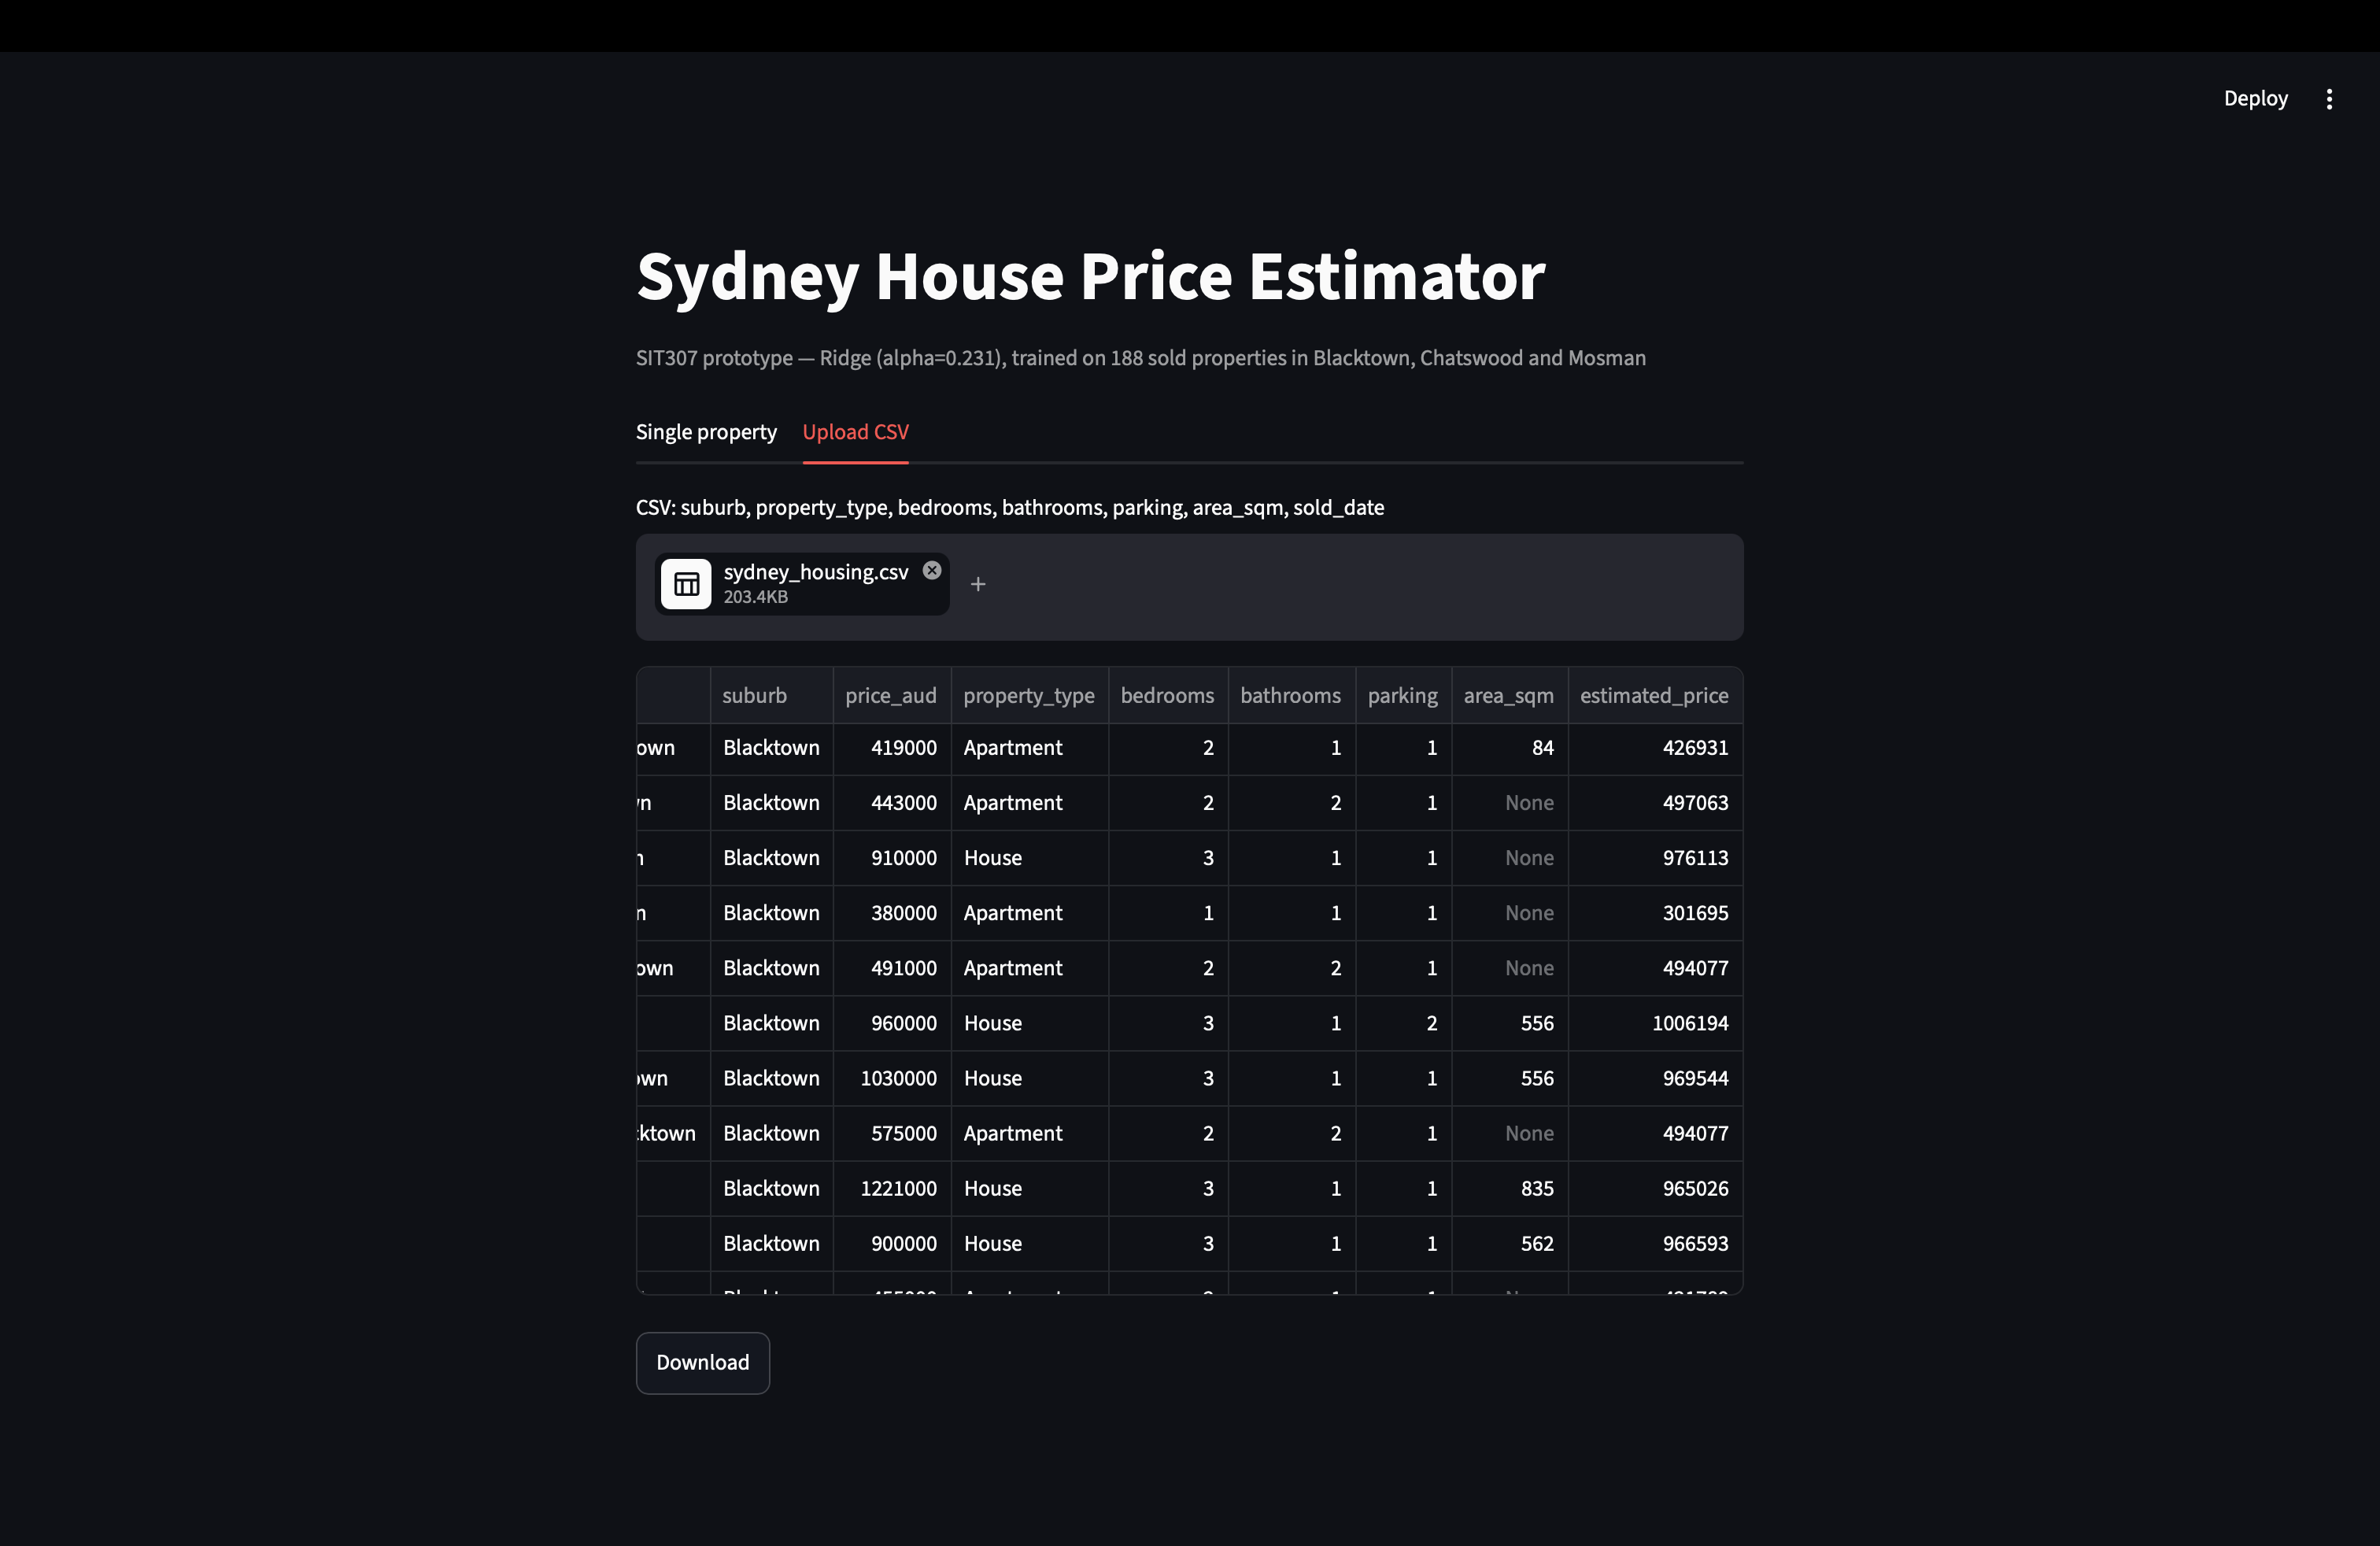
\includegraphics[width=\linewidth]{figures/p5_app_csv.png}
\caption{Batch estimates from an uploaded CSV.}\end{subfigure}
\caption{The Streamlit application. Estimates are shown with a $\pm 20\%$ band, and
warnings fire on the cases Section~4 identified as unreliable.}
\label{fig:app}
\end{figure}


\subsection{Reflection}

\textbf{Data collection was the real bottleneck, not modelling.} Only 188 of the 239
listings passed the completeness rule, and almost every later limitation comes back to
that number. The learning curves were still improving at the end, so more sales would
have helped more than a better estimator. Choosing which rows to drop also turned out to
be a modelling decision. Exempting \texttt{area\_sqm} kept the suburbs balanced, but
it meant imputing that column for a third of the sample.

\textbf{Evaluation choices changed the conclusions.} When we scored in-sample instead of
out-of-fold, the top two models swapped places. Likewise, MAPE computed on the logged
target read 1.17\% rather than the actual 16.8\%.

\textbf{Accuracy versus deployability.} Noticeably, the most useful signals were also the
hardest to serve. Since \texttt{area\_sqm} is a third missing, the application has to
accept a blank and fall back on the training median, while the \texttt{kw\_*} flags
added almost nothing. Therefore, the deployed model only asks for fields that can be read
off a listing in seconds, and we accept about $\pm 20\%$ error in exchange for an
interface that needs no preparation.

\textbf{Bias and fairness.} Three suburbs do not represent Sydney, and even within them
coverage is uneven, with 79 Blacktown sales against 47 in Mosman. The error follows the
same pattern, at 11.7\% against 20.9\%. Moreover, suburb is an explicit input and SEIFA
turned out to be the suburb label restated, so the model encodes existing spatial
inequality and would carry it into any decision it informs.

\textbf{Given more resources.} First, a longer collection window would separate
seasonality from trend and fill in the sparse Mosman tail. Second, capturing
\texttt{area\_sqm} at collection time would remove the need to impute it. Finally,
nested cross-validation would remove the optimism still left in the CV figures.

